\section{Additional Topics - 额外主题}
\subsection{Introduction to Quantum Circuits and Quantum Computing - 量子电路和量子计算初探}
Consider an $n$-qubit system with $\hilbert = (\C^2)^{\otimes n} = \C^{2^n}$. A quantum circuit with $n$ qubits can be the following:
\begin{center}
    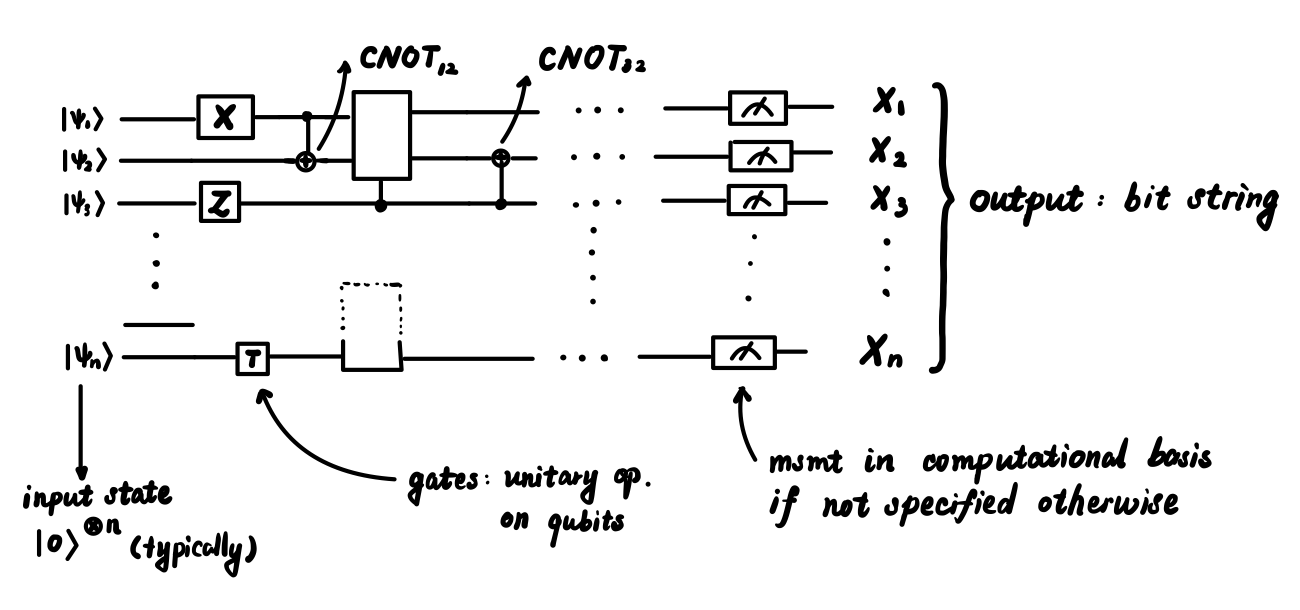
\includegraphics[scale = 0.6]{qcircuit.png}
\end{center}
If we want to measure in a different basis, say the columns of a unitary operator $V$, then one can apply $\conjt{V}$ before the measuring in the computational basis instead. \\
The final measurement give one bitstring per run of the circuit, and good quantum algorithms only need a few runs and results. \\
Discrete gates are typically implemented by turning on and off interactions (lasers, microwave pulses, bringing qubits closer to each other through Coulomb force). Take Pauli-X gate as an example, the Hamiltonian is $H_{\text{int}} = \alpha X$, which gives the unitary propagator to be:
$$\opuni(t) = \exp(-\frac{\imag \alpha X t}{\hbar}) = \cos(\frac{\omega t}{2})\id - \imag \sin(\frac{\omega t}{2})X$$
where $\omega = \frac{\alpha}{\hbar}$. If the interaction acts for $\Delta t = \frac{\pi}{\omega} = \frac{\pi \cdot \hbar}{\alpha}$, then, $\opuni(\Delta t) = (-\imag)X$. \par
Like a classical circuit, the quantum gates play an important role. Consider the controlled gates, an example is the CNOT gate:
\begin{align*}
    \text{CNOT}: \ket{00} &\mapsto \ket{00} \\\
    \ket{01} &\mapsto \ket{01} \\
    \ket{10} &\mapsto \ket{11} \\
    \ket{11} &\mapsto \ket{10}
\end{align*}
A general controlled-$\opuni$ gate would be:
\begin{align*}
    \text{C-}\opuni: \ket{00} &\mapsto \ket{00} \\\
    \ket{01} &\mapsto \ket{01} \\
    \ket{10} &\mapsto \ket{1} \otimes \opuni\ket{0} \\
    \ket{11} &\mapsto \ket{1} \otimes \opuni\ket{1}
\end{align*}
We further wish to know what total unitaries can be implemented on quantum circuits (a unitary that acts on all $n$ qubits). With a universal set of elementary gates, any $\opuni_{\text{tot}} \in \opuni((\C^2)^{\otimes n})$ can be implemented. In \impt{classical computation}, a universal set of gates is the $\{\text{NAND}\}$, that is, if the NAND gate is implemented, any logical operators can be implemented. In quantum computation, some known universal sets are:
\begin{quote}
    1. $\{T, H, \text{CNOT}\}$, where $H$ is the Hadamard, and
    $$T = \begin{pmatrix}
        1 & 0 \\ 0 & \exp(\frac{\imag \pi}{4})
    \end{pmatrix}$$
    This set can approximate any $\opuni_{\text{tot}}$ \impt{up to arbitrary precision}. \\
    2. $\{H, \text{Toffoli}\}$, the Toffoli is controlled-CNOT gate (only applying NOT when the first two qubits are both $\ket{1}$). \\
    3. Note that $\{X, Y, Z, H, CNOT, S\}$ is \impt{not universal}, where
    $$S = \begin{pmatrix}
        1 & 0 \\ 0 & \imag
    \end{pmatrix}$$
\end{quote}
The next question becomes what total unitaries can be implemented efficiently (with $\text{poly}(n)$ elementary gates). And this remains a challenge to find \impt{useful, efficient, and implementable} total unitaries. An example of such findings is Shor's integer factorization algorithm, which factorizes an integer $N$ into two prime numbers $p, q$ so that $N = pq$.

\subsection{Quantum Entanglement - 量子纠缠}
Maximally entangled states (a.k.a Bell states) of $2$ qubits in $\hilbert = \C^2 \otimes \C^2$ are:
\begin{align*}
    \ket{\psi^{00}} &= \frac{1}{\sqrt{2}}(\ket{00} + \ket{11}) = \ket{\Phi^{+}} \\
    \ket{\psi^{01}} &= \frac{1}{\sqrt{2}}(\ket{00} - \ket{11}) = \ket{\Phi^{-}} \\
    \ket{\psi^{10}} &= \frac{1}{\sqrt{2}}(\ket{01} + \ket{10}) = \ket{\Psi^{+}} \\
    \ket{\psi^{11}} &= \frac{1}{\sqrt{2}}(\ket{01} - \ket{10}) = \ket{\Psi^{-}} \\
\end{align*}
These states form an orthonormal basis of $\hilbert$ and the measurements in these basis are called \impt{Bell measurements}. These states have the following properties:
\begin{quote}
    1. $\forall i, j \in \{0, 1\}$, $\tr_B(\dyad{\psi^{ij}}) = \frac{1}{2}\id_A$ and $\tr_A(\dyad{\psi^{ij}}) = \frac{1}{2}\id_B$. \\
    2. Local interconvertibility: $\ket{\psi^{ij}} = (-1)^{ij} \cdot \id_A \otimes (X_B^iZ_B^j)\ket{\psi^{00}}$
\end{quote}
The quantum circuit for preparing $\ket{\psi^{ij}}$ is:
\begin{center}
    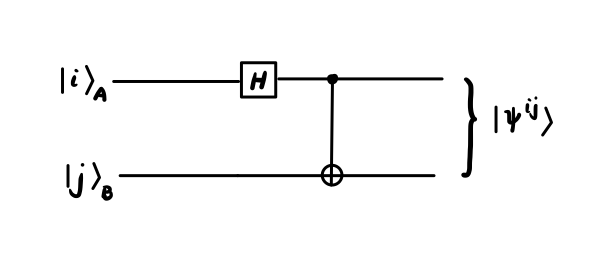
\includegraphics[scale = 1]{bell.png}
\end{center}
The Bell states are often used as a basis resource in quantum information protocols (quantum teleportation, quantum key distribution, entanglement enhanced ``abc'' - protocols).
\subsubsection{Distinction between Entangled States and Mixed States}
A bipartite state $\rho_{AB} \in \rho(\hilbert_A \otimes \hilbert_B)$ is called:
\begin{quote}
    1. a product state, if $\rho_{AB} = \rho_A \otimes \rho_B$, and $\rho_A \in \mathcal{S}(\hilbert_A), \rho_B \in \mathcal{S}(\hilbert_B)$. \\
    2. a \impt{separable} state, if $\displaystyle \rho_{AB} = \Sumi{k} q_k \rho_A^{(k)} \otimes \rho_B^{(k)}$.
    $$\rho_{AB} = \frac{1}{5} \dyad{+}\otimes\dyad{0} + \frac{4}{5}\dyad{0}\otimes\dyad{-}$$
    3. an entangled state, if $\rho_{AB}$ is not separable.
\end{quote}
\begin{definition}
    \uimpt{Werner states} are states $\rho_{AB} = \lambda \dyad{\psi^{01}} + (1-\lambda)\frac{\id_4}{4}$, where $\lambda \in [0,1]$. It can be shown that Werner states are entangled when $\lambda > \frac{2}{3}$.
\end{definition}

\subsection{Quantum Teleportation - 量子遥传}
The setting of quantum teleportation is the following:
\begin{quote}
    1. Two agents (Alice and Bob) are placed in different locations. \\
    2. They share a maximally entangled state, say $\ket{\psi^{00}}_{AB}$. \\
    3. They can exchange classical bits. \\
    4. Alice holds a qubit $S$, where $\ketpsi_S = \alpha\ket{0}_S + \beta\ket{1}_S$.
\end{quote}
The goal is to ``teleport'' $\ketpsi_S$ to Bob's system, or preparing $\ketpsi_B$ on $B$ by only exchanging classical information.
\begin{center}
    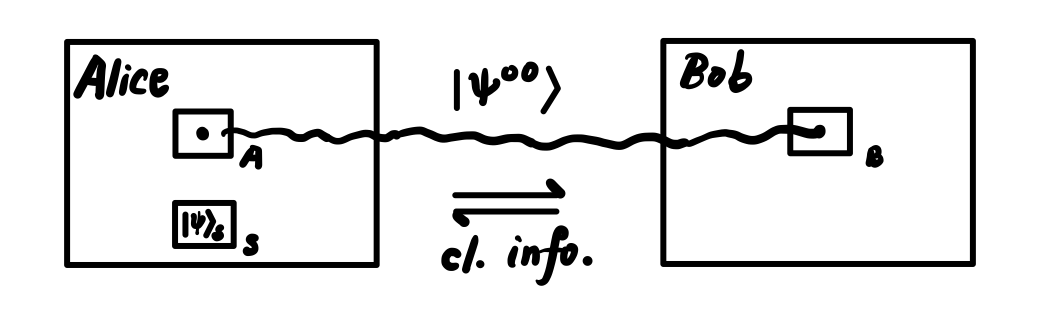
\includegraphics[scale = 0.8]{qtele-setup.png}
\end{center}
The protocol is as follows:
\begin{center}
    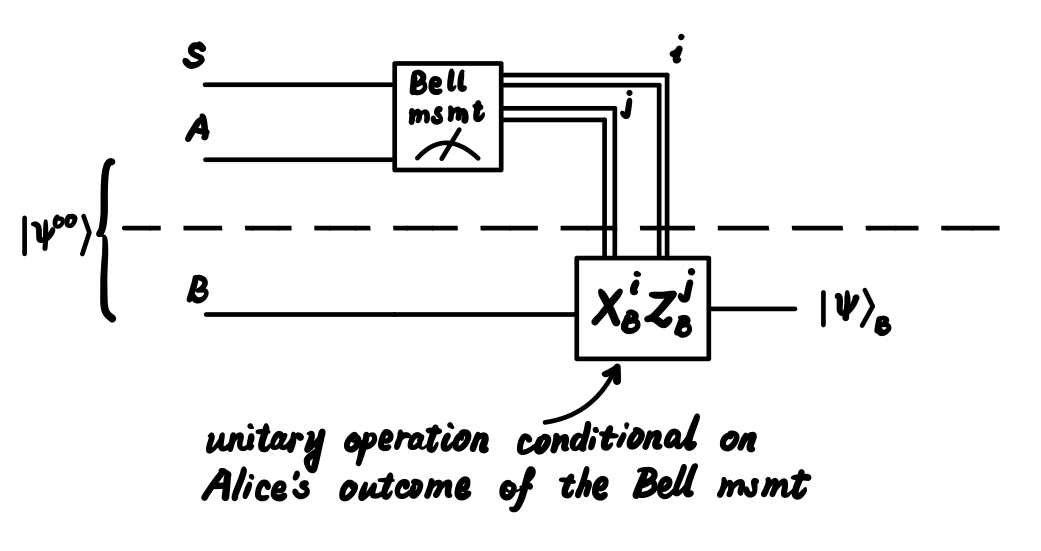
\includegraphics[scale = 0.8]{qtele-protocol.png}
\end{center}
where the Bell measurement is inversed in this case:
\begin{center}
    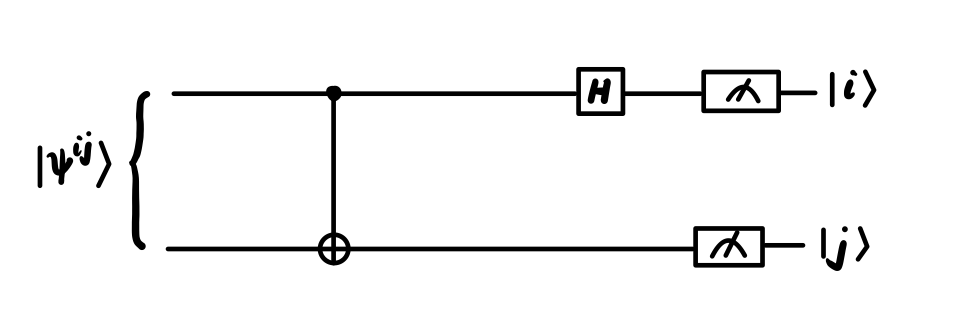
\includegraphics[scale = 0.8]{bell-inverse.png}
\end{center}
We now analyze this circuit. Suppose the initial state to be:
\begin{align*}
    \ketPsi_{SAB} &= \ketpsi_S \otimes \ket{\psi^{00}}_{AB} \\
    &= (\alpha \ket{0} + \beta \ket{1})_S \otimes \frac{1}{\sqrt{2}}(\ket{00}_{AB} + \ket{11}_{AB}) \\
    &= \frac{\alpha}{2}\ket{000} + \frac{\alpha}{011} + \frac{\beta}{2}\ket{100} + \frac{\beta}{2}\ket{111}
\end{align*}
Further suppose the outcome from the inverse Bell measurement $i = 1, j = 0$ is obtained, then the post-measurement state on $SAB$ is:
\begin{align*}
    \ket{\Psi_{(1, 0)}'}_{SAB} &= \frac{1}{\text{norm.}}(\dyad{\psi^{10}}\otimes \id_B)\ketPsi_{SAB} \\
    &= \ket{\psi^{10}} \otimes (\alpha \ket{1} + \beta\ket{0})
\end{align*}
Bob now applies $X_B^1Z_B^0 = X_B$, the final state on $B$ will be:
$$X_B(\alpha \ket{1} + \beta\ket{0}) = \alpha \ket{0} + \beta\ket{1}$$
Note that, quantum teleportation works independently of $\alpha, \beta \in \C$, hence it also works these values are unknown. The transmission of $2$ classical bits is necessary and optimal, without knowing $(i, j)$, Bob's state is maximally mixed. The classical analogue is rather straightforward, that is transmitting a classical bit from $A$ to $B$. Without knowing the bit initially, we simply look at the bit to know the value and sent it across. This is not useful for qubits because a measurement on $S$ alone does not allow us to know $\alpha, \beta$.


\subsection{No-cloning Theorem - 不可克隆原理}
The na\"ive idea for ``quantum teleportation'' is to copy $\ketpsi$ many times, and measure the copies to obtain good estimates for $\alpha, \beta$, then send these values as classical information for Bob to prepare. However, this does not work. 
\begin{definition}
    Consider two quantum systems $\hilbert_A \cong \hilbert_B$, a \uimpt{quantum cloning operation} on $\hilbert_A$ is a process that achieves:
    $$\forall \ketpsi_A \in \hilbert_A, \ketpsi_A\ket{0}_B \mapsto \ketpsi_A\ketpsi_B$$
\end{definition}
Note that CNOT is not a cloning operation because:
$$\ketplus_A \ket{0}_B \mapsto \ket{\psi^{00}} \ne \ketplus_A\ketplus_B$$
\begin{theorem}
    The \uimpt{no-cloning theorem} states that it is impossible to clone an unknown quantum state.
\end{theorem}
The proof for this theorem is as follows: \\
A cloning process would have to achieve
\begin{center}
    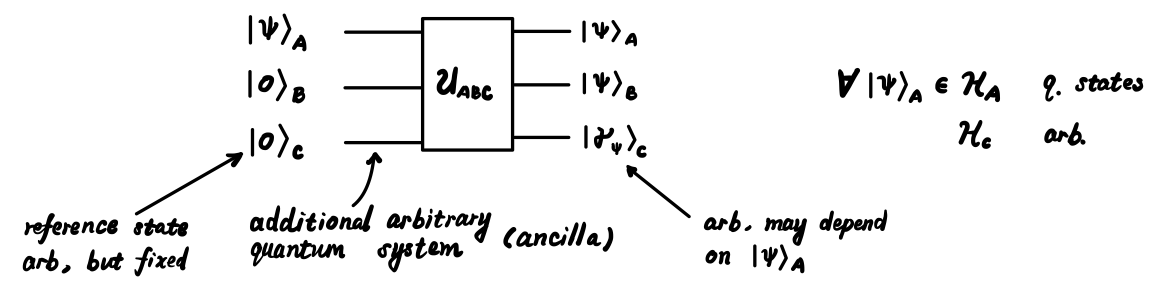
\includegraphics[scale = 0.75]{clone.png}
\end{center}
Consider another state $\ketphi_A \in \hilbert_A$ where $0 < \abs{\braket{\psi}{\psi}} < 1$. Recall that unitary operators should \impt{preserve inner products}, then we have:
\begin{align*}
    \abs{\braket{\psi 0 0}{\phi 0 0}} &= \abs{\braket{\psi}{\phi}_A} \\
    \abs{\braket{\psi\psi\gamma_\psi}{\phi \phi \gamma_\phi}} &= \abs{\braket{\psi}{\phi}_A} \cdot \abs{\braket{\psi}{\phi}_B} \cdot \abs{\braket{\gamma_\psi}{\gamma_\phi}_C} \\
    &\le \abs{\braket{\psi}{\phi}_A}^2
\end{align*}
However, $\abs{\braket{\psi}{\phi}_A} > \abs{\braket{\psi}{\phi}_A}^2$, by it being between $0$ and $1$, we see that it contradicts with the unitary preserving inner products. \\
Note that the evolutions in nature are all unitary evolutions, it is crucial to see that they are linear operations. And the key reason why cloning is impossible is that it is not a linear operation. \\
The no-cloning theorem thus implies that there is no na\"ive quantum teleportation; there is no na\"ive quantum error correction protocol; it is the basis of security proofs for quantum cryptography (quantum key distribution); and it implies monogamy of non-classical correlations. \\
Specifically, for error correction protocol, this prevents us from doing:
$$\ketpsi = \alpha \ket{0} + \beta \ket{1} \mapsto (\alpha \ket{0} + \beta \ket{1})^{\otimes n}$$
and we do this instead:
$$\alpha \ket{0} + \beta \ket{1} \mapsto \alpha\ket{000} + \beta\ket{111}$$
\begin{center}
    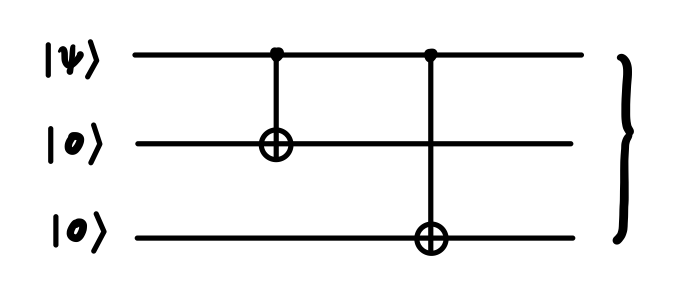
\includegraphics[scale = 1]{error-correction.png}
\end{center}
Furthermore, specifically for quantum cryptography, consider the situation where there exists an ``Eve'' who wishes to know the key between Alice and Bob, then:
\begin{center}
    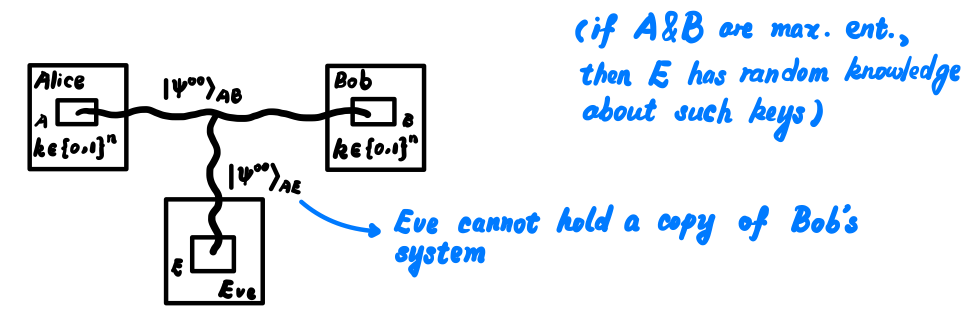
\includegraphics[scale = 0.75]{quantum-security.png}
\end{center}
Eve is being prevented from knowing the key because if Eve forms such entangled states, she would have an exact copy of Bob's system. Only Eve or Bob (one person) can be maximally entangled with Alice, but not both.
\begin{definition}
    \uimpt{Monogamy of non-classical correlations} means if two parties are correlated to the maximal extent possible, then they cannot be correlated with any other system in the world.
\end{definition}
\bigskip
\begin{center}
    {\huge \textbf{Marchons, marchons !}}
\end{center}